% Battery dispatch: offline value learning and online mixed-integer control.
\documentclass[preprint,11pt]{elsarticle}

\usepackage[T1]{fontenc}
\usepackage{lmodern}
\usepackage[utf8]{inputenc}
\usepackage{amsmath,amssymb,amsfonts,amsthm,mathtools,bm}
\usepackage{booktabs,graphicx,tabularx,array}
\usepackage{enumitem}
\usepackage{setspace}
\usepackage{placeins}
% SMPT: square-bracket numeric citations in order of first appearance.
% The official elsarticle-num-names style also supports Author [number].
\usepackage[american]{babel}
\biboptions{numbers,sort&compress}

\usepackage[colorlinks=true,linkcolor=blue,citecolor=blue,urlcolor=blue]{hyperref}
\pdfstringdefDisableCommands{\def\corref#1{}}

\DeclareMathOperator*{\argmin}{arg\,min}
\newcommand{\R}{\mathbb{R}}
\newcommand{\E}{\mathbb{E}}
\newcommand{\cA}{\mathcal{A}}
\newcommand{\cX}{\mathcal{X}}
\newcommand{\cT}{\mathcal{T}}
\newcommand{\osc}{\operatorname{osc}}
\newcommand{\norm}[1]{\left\lVert #1\right\rVert}
\newcommand{\abs}[1]{\left\lvert #1\right\rvert}

\theoremstyle{plain}
\newtheorem{proposition}{Proposition}
\newtheorem{corollary}{Corollary}
\theoremstyle{remark}
\newtheorem{remark}{Remark}

\journal{Simulation Modelling Practice and Theory}
\emergencystretch=3em
% Keep substantial result floats with surrounding discussion in the preprint.
\renewcommand{\topfraction}{0.9}
\renewcommand{\bottomfraction}{0.8}
\renewcommand{\textfraction}{0.08}
\renewcommand{\floatpagefraction}{0.8}

\begin{document}

\begin{frontmatter}

\title{Simulation-based comparison of offline value learning and online
mixed-integer control for battery dispatch}

\author[aff1]{Yeoneung Kim\corref{cor1}}
\ead{yeoneung@yonsei.ac.kr}
\cortext[cor1]{Corresponding author}
\affiliation[aff1]{organization={Department of Industrial Engineering, Yonsei University},
             addressline={50 Yonsei-ro, Seodaemun-gu},
             city={Seoul},
             postcode={03722},
             country={Republic of Korea}}

\begin{abstract}
We use a common simulation model to compare offline stochastic value learning
with online mixed-integer model predictive control for battery dispatch
under a discontinuous import-band fee.
All controllers share the economic objective, terminal treatment, information,
15-minute update interval, and feasible set. The learned controller combines
smooth finite-horizon training with hard-cost one-step action selection.
Comparators are conditional-mean and two-stage stochastic exact-band
mixed-integer quadratic programs (MIQPs) under explicit solve budgets.
A discrete Bellman bound separates approximation and implementation errors.
Evaluation uses a fixed train--validation--test
split, four seasons, and threshold--fee--smoothing sensitivity.
On 30 held-out 2019 winter weekdays, its mean cost was 1.2\% higher, 2.3\% higher, and 1.4\% higher relative to the lower-cost online MIQP at fee rates of 20, 40, and 80 EUR/h, respectively. The prespecified learned-superiority rule was met in 1 of six MIQP comparisons. Central-fee inference resampled five independent five-restart batches; each outer-anchor result is conditional on one such batch. Its mean GPU-assisted online latency was 3.1 ms versus 1054.9 ms for single-threaded conditional-mean MIQP.
The learned correction reduces cost by 2.9\%, 11.9\%, and 24.6\% relative to a
matched reference-only controller with the same hard-cost decision rule.
\end{abstract}

\begin{keyword}
Simulation benchmarking \sep approximate dynamic programming
\sep model predictive control \sep mixed-integer optimization
\sep stochastic control \sep battery dispatch
\end{keyword}

\end{frontmatter}
\onehalfspacing

\section{Introduction}\label{sec:introduction}

An operator deciding battery power every few minutes can either solve a new
optimization problem online or evaluate a policy learned offline. The first
approach adapts naturally to current forecasts but repeatedly consumes solver
time. The second shifts computation away from operations but introduces
approximation, training variability, and model risk. This trade-off is most
consequential when the operating cost is discontinuous. A fee triggered by
crossing an import band, for example, creates a decision boundary that a convex
surrogate can move or remove.

Simulation provides a controlled setting for comparing these approaches, but
the comparison depends on how each controller is implemented and evaluated.
In particular, training on a smooth objective and deploying actions under a
discontinuous tariff can introduce differences that are absent from the
training model. Separating these effects from the contribution of learning
requires both numerical checks and matched controller comparisons.

Both approaches are well established. Rolling-horizon model predictive control
(MPC) is widely
used for microgrid and storage scheduling \citep{Parisio2014,Zhang2022}.
Stochastic dual dynamic programming, approximate dynamic programming, and
parametric lookahead policies shift some or all computation offline
\citep{Pereira1991,Lohndorf2010,Jiang2015,Powell2019}. In closely related work,
\citet{Ghadimi2024} learn parameters of a storage lookahead model under evolving
forecasts. \citet{Gust2021} compare forecast-based and reactive microgrid
strategies under demand charges, export limits, and forecast error,
highlighting the importance of control intervals in strategy comparisons.
Neural PDE methods provide another route to
continuous-state value functions \citep{Sirignano2018,Raissi2019}, and policy
iteration separates a
linear policy-evaluation equation from pointwise policy improvement
\citep{Kerimkulov2020}.

A practical comparison must account for offline training and restart
selection as well as online solver time. It must also match update rates,
forecast information, horizons, and terminal treatment. Otherwise, apparent
performance differences may reflect different decision problems. Near the
threshold, a smooth neural objective can additionally rank actions differently
from the hard tariff used for settlement.

This paper develops a simulation-based comparison of offline value learning
and online optimization under a common dispatch model, objective, and
information structure. It asks how much learned continuation values improve
dispatch and how this improvement compares with the cost and computation of
online optimization. Deployment consistency links the controller design to
the evaluation protocol. All
main controllers are updated every 15 minutes, evaluated under one hard
economic objective, and charged the same soft terminal cost. The learned value
does not directly determine the held action through a smooth Hamiltonian.
Instead, a one-step hard-cost problem is solved over the deployed feasible set,
including the tariff crossing. Learned checkpoints and restarts are selected
by validation-period economic cost, never by a residual alone.

The study has three main components.
First, it gives a common simulation benchmark for offline feedback and online exact-band
optimization, with matched objectives, information, terminal treatment, and
computational accounting. Conditional-mean and two-stage stochastic
mixed-integer quadratic programs (MIQPs) are complemented by tariff-surrogate
and no-learning controls. Nested sets of 2, 8, and 16 paths over three
independent streams assess scenario resolution under explicit solve budgets.
Second, it develops a deployment-consistent learned
controller. A no-storage reference value removes an economically known part of
the approximation problem, while its no-learning counterpart isolates the
economic contribution of the learned correction. Hard-cost one-step
improvement accounts for the held-action interval, safety bounds, reflection,
and the discontinuous fee.
Third, a finite-horizon Bellman analysis organizes approximation and
implementation errors for the action actually held after deployment logic.
Numerical checks, seasonal replay, tariff sensitivity, and separate offline
and online timing measurements then assess decision accuracy and the
cost--computation trade-off.

The distinction from recent neural policy-iteration theory is direct.
\citet{Meng2024} analyze deterministic infinite-horizon control-affine systems
with quadratic control, whereas \citet{Kim2025} analyze stationary second-order
stochastic HJB equations and interior errors of bounded-domain policy
evaluation. Our contribution addresses finite-horizon operational control by
aligning approximation diagnostics with discrete held actions and a hard tariff.

\section{Simulation model and common decision protocol}\label{sec:benchmark}

\subsection{State, observations, and battery dynamics}

The operating day is divided into $K=96$ intervals of length
$\Delta=0.25$ hours. At time $t_k=k\Delta$, the controller observes
$X_k=(S_k,Y_k,P_k)$: state of charge (SoC), net-load error, and price error.
Calendar regime $r$ determines hourly median profiles $\bar n_r(t)$ and
$\bar c_r(t)$, so observed net load and price are
\begin{equation}
 N_k=\bar n_r(t_k)+Y_k, \qquad C_k=\bar c_r(t_k)+P_k.
\end{equation}
The action $A_k$ is positive for discharge and negative for charge; write
$z^{\pm}=\max\{\pm z,0\}$. With
energy capacity $E_{\max}$ and efficiencies $\eta_c,\eta_d$,
\begin{equation}
 S_{k+1}=S_k+\frac{\Delta}{E_{\max}}
 \left(\eta_c A_k^- - \frac{A_k^+}{\eta_d}\right).
 \label{eq:soc-transition}
\end{equation}
Grid exchange is $G_k=N_k-A_k$, with positive values denoting import.

Power tapers near the SoC limits. Let
\begin{align}
 q_c(s)&=\min\left\{1,\frac{s_{\max}-s}{\delta_s}\right\}, &
 q_d(s)&=\min\left\{1,\frac{s-s_{\min}}{\delta_s}\right\},\\
 \cA_{\mathrm{cont}}(s)
   &=\left[-\bar a_cq_c(s),\,\bar a_dq_d(s)\right].
\end{align}
The held action must also keep the next SoC feasible under
\eqref{eq:soc-transition}. This gives
\begin{equation}
 \cA_{\Delta}(s)=\left[
 -\min\left\{\bar a_c,\frac{E_{\max}(s_{\max}-s)}{\eta_c\Delta}\right\},
 \min\left\{\bar a_d,\frac{\eta_dE_{\max}(s-s_{\min})}{\Delta}\right\}
 \right]
\end{equation}
and the deployed interval
\begin{equation}
 \cA_{\mathrm{dep}}(s)=\cA_{\mathrm{cont}}(s)\cap\cA_{\Delta}(s).
 \label{eq:deployed-set}
\end{equation}
Every main method optimizes over or maps directly into this same interval.

For offline modeling, $(Y,P)$ follow correlated mean-reverting diffusions on
a training-period box. Simulation uses exact OU steps followed by reflection.
Before reflection, the regime-specific dynamics are
\begin{equation}
 \begin{aligned}
 dY_t&=-\kappa_yY_t\,dt+\sigma_y\,dW_t^y,\\
 dP_t&=-\kappa_pP_t\,dt+\sigma_p\,dW_t^p,\\
 d\langle W^y,W^p\rangle_t&=\rho\,dt.
 \end{aligned}
 \label{eq:ou-model}
\end{equation}
The conditional-mean MPC forecast uses the usual unreflected exponential mean.
It is therefore an approximation near the boundary, not the exact mean of the
reflected process. Section~\ref{sec:mechanisms} measures this difference and
reports how often historical observations require reflection.
The observed current net load and price enter the first-stage cost unchanged;
reflected residuals condition the continuation model, not the current bill.

\subsection{Common economic objective}

All reported methods use the same hard stage cost
\begin{align}
 c_k(x,a)=\Delta\big[&C_kG_k^+-\alpha_s C_kG_k^-
 +\lambda_1\abs{a}
 +c_f\mathbf 1\{G_k>G_{\mathrm{thr}}\}\big],
 \label{eq:hard-stage}
\end{align}
and terminal cost
\begin{equation}
 \Phi(S_K)=\lambda_T(S_K-s_{\mathrm{tar}})^2.
 \label{eq:terminal}
\end{equation}
Thus
\begin{equation}
 J^\pi_k(x)=\E_x^\pi\left[
 \sum_{j=k}^{K-1}c_j(X_j,A_j)+\Phi(S_K)\right].
 \label{eq:common-objective}
\end{equation}
The coefficients $\lambda_1$ and $\lambda_T$ are fixed from training-period
scale. The objective contains no quadratic peak, quadratic action, or
SoC-centering regularization terms. The band indicator,
positive parts, and absolute throughput are exact in selection and evaluation.
Smoothing is confined to neural training and is varied as a mechanism check.

This fee is a controlled threshold-tariff benchmark rather than a claim about
a specific retail contract. Fee rate, threshold, and battery scale are stated
in full so the economic experiment can be reproduced. The primary threshold is
300 kW, the training width is 10 kW, and fee rates are 20, 40, and 80 EUR/h.

\subsection{Online-optimization comparators}

The deterministic comparator is a shrinking-horizon exact-band MIQP. At every
15-minute epoch it uses the current error and its OU conditional mean, exact
transaction and throughput terms, binary variables for the band indicator,
and the common quadratic terminal cost. Charge/discharge and import/export
logic is enforced at every price, including in time-limited incumbents. The
label \emph{exact-band} refers to the tariff representation, subject to the
documented binary separation and numerical action recovery. A solve
is not labeled optimal unless the solver proves it; relative gaps, time limits,
and missing incumbents are reported separately.

To isolate tariff representation, a matched comparator replaces the band fee
by a convex hinge. On the calibrated interval $G\leq G_{\max}$, its slope is
$c_f/(G_{\max}-G_{\mathrm{thr}})$, so the hinge is a convex lower envelope of
the flat fee. Forecast, horizon, terminal cost, constraints, and update timing
are otherwise unchanged. Evaluation still charges the hard fee in
\eqref{eq:hard-stage}. Direction binaries are retained at every forecast
price to prevent simultaneous flows; hence ``convex envelope''
describes the tariff surrogate rather than every auxiliary constraint.

The stochastic comparator draws reflected OU scenarios conditional on the same
observation. Its current charge and discharge variables are shared across all
scenarios, while future decisions are scenario-contingent. It is therefore a
two-stage approximation with a nonanticipative first action. Its larger model
is computationally demanding, while its scenario-contingent future recourse
uses more information than a feasible multistage policy and makes the lookahead
objective optimistic. A
feasible no-storage solution is supplied as a primal start to the larger
scenario model. If either exact-band solve returns no incumbent, the controller
holds zero action for that interval. Incumbent availability and fallback use
are retained in the solver record. Both MIQPs reoptimize at 15-minute epochs.

No storage is retained as a scale reference. The exact-band formulations are
the primary online comparators; the envelope formulation isolates the value of
the discontinuous tariff representation. A price-threshold rule, whose charge
and discharge thresholds are selected from training-price quantiles on the
same validation days, provides a low-dimensional baseline; no action is one
candidate. The comparator family uses information available at dispatch.
Actor--critic methods such as SAC and TD3 \citep{Haarnoja2018,Fujimoto2018}
offer a separate comparison between learned-feedback pipelines. Here we focus
on matched online optimization and use an independent numerical dynamic
program for the low-dimensional approximation check in Section~\ref{sec:gate}.

\section{Deployed offline value policy}\label{sec:method}

\subsection{Smooth value approximation and reference policy}

The offline learner uses the continuous-time generator associated with
\eqref{eq:soc-transition} and the fitted OU model. Training smooths the
positive parts, throughput absolute value, and band indicator. It alternates
approximate solution of the linear fixed-policy backward equation with scalar
Hamiltonian search over $\cA_{\mathrm{dep}}(s)$: a coarse grid split at zero,
followed by refinement on each sign interval. The loss includes residual and
reflecting-boundary derivative penalties, detailed in the supplement.

Nonconvexity alone does not invalidate exact policy iteration. With exact
policy evaluation and sufficient regularity or a valid verification argument,
an admissible Hamiltonian-improving update yields the policy-improvement
inequality without requiring convexity in the action. Nonconvexity instead
complicates minimization: a local stationary point alone does not establish
global greediness. Here, neural evaluation and numerical search are
approximate; the convergence assumptions of classical policy-iteration theory
\citep{Kerimkulov2020} are not asserted for the full training and deployment
procedure.

Rather than learn the full value from the terminal quadratic, the network uses
\begin{equation}
 v_\theta(t,x)=V^{0}_{\mathrm{cm}}(t,x)
 +(T-t)\beta N_\theta(\widetilde t,\widetilde x),
 \label{eq:reference-ansatz}
\end{equation}
where $V^{0}_{\mathrm{cm}}$ approximates the no-storage cost-to-go along the
OU conditional-mean path. Midpoint quadrature evaluates this
reference, and tildes denote affine normalization to $[-1,1]$. This structured
baseline leaves the neural network to approximate the correction. The final network
layer is initialized at zero, so training starts from $V^{0}_{\mathrm{cm}}$
rather than a large random correction. The scale $\beta$ is specific to the
correction and is checked together with physical-coordinate derivatives.
Equation~\eqref{eq:reference-ansatz} enforces \eqref{eq:terminal} exactly.

We assess the approximation through value error, action error, sign
disagreement, local Hamiltonian regret, and the cost of the frozen policy
on an independent finite-difference reference. Economic validation, rather
than the training residual, determines checkpoint and restart selection.

\subsection{Reference-only counterfactual and hard-cost deployment}

Let $R_k=V^0_{\mathrm{cm}}(t_k,\cdot)$ denote the fixed reference term in
\eqref{eq:reference-ansatz}. To separate the neural correction from the
one-step decision architecture, define the no-learning controller
\begin{equation}
 \pi_k^{\mathrm{ref}}(x)\in\argmin_{a\in\cA_{\mathrm{dep}}(s)}
 \left\{c_k(x,a)+
 \E[R_{k+1}(X_{k+1})\mid X_k=x,A_k=a]\right\}.
 \label{eq:reference-controller}
\end{equation}
The error transition is action-independent, and the no-storage running part
of $R_{k+1}$ is independent of SoC under the common objective. Thus the only
action-dependent continuation term in \eqref{eq:reference-controller} is
$\lambda_T(S_{k+1}-s_{\mathrm{tar}})^2$. The implementation minimizes the
hard current stage cost plus this terminal term on exactly the same candidate
set used by the learned controller. This is an active dispatch rule, not the
zero-action or no-storage baseline. It differs from learned deployment only by
removing $(T-t)\beta N_\theta$, so their paired cost difference attributes the
incremental value of the learned continuation correction.

Training uses a smooth continuous-time Hamiltonian; deployment instead
numerically approximates the discrete hard-cost one-step decision
\begin{equation}
 \pi_k^{v_\theta}(x)\in\argmin_{a\in\cA_{\mathrm{dep}}(s)}
 \left\{c_k(x,a)+
 \E\left[v_\theta(t_{k+1},X_{k+1})\mid X_k=x,A_k=a\right]\right\}.
 \label{eq:one-step}
\end{equation}
The deployed policy approximates this target using fixed Gauss--Hermite
quadrature for the correlated OU step with reflection.
The action grid is confined to the deployed interval before evaluation. It
includes both endpoints, zero, the crossing
$a=N_k-G_{\mathrm{thr}}$, and feasible candidates with fee-side membership
verified after computing $N_k-a$. A denser independent grid audits the search
defect. Proposition~\ref{prop:grid-defect} concerns this hard-cost deployment
search, not the smooth Hamiltonian search used during training.

At $k=K-1$, the next value in \eqref{eq:one-step} is exactly the common
terminal cost. This feature prevents a continuous-time gradient error from
creating a different terminal convention. A final projection is
retained as a numerical guard. Native clipping leaves every already feasible
action unchanged, including its floating-point representation. Billing uses
the strict indicator in \eqref{eq:hard-stage}, without an exceedance tolerance.
For an MIQP incumbent with an inactive band binary, a first-action overshoot
within the documented $10^{-5}$-kW separation may be recovered to a verified
feasible crossing before deployment; the correction and actual held action
are logged. Cost is always recomputed from that held action.

\subsection{Economic selection and complete procedure}

For each primary
anchor and seasonal cell, training produces five independent restarts; the
noncentral factorial cells use one restart and remain descriptive. Within each
restart,
candidate PI checkpoints are evaluated on the same validation days under
\eqref{eq:hard-stage}--\eqref{eq:terminal}. Starting from the first candidate,
the incumbent changes only if paired mean cost improves by at least 0.10
EUR/day. The residual is retained as a diagnostic and tie description, not the
selection objective.

The five checkpoint winners then enter a sequential validation rule whose
initial incumbent is the feasible zero-action policy. A learned policy replaces
the incumbent only by the same 0.10 EUR/day margin. Thus five restarts, two
levels of validation selection, the fallback, hard one-step action, and the
safety layer form one algorithm. The central fee cell uses five independent
five-restart batches to
expose batch-to-batch selection variation. Checkpoints and restarts are selected
on validation data; no width is selected by test cost. Solver budgets and the
escalation rule are recorded before the corresponding additional runs.

Each five-restart deployment follows four steps:
\begin{enumerate}[label=\arabic*.,leftmargin=2em,itemsep=1pt,topsep=3pt]
 \item fit profiles, OU parameters, bounds, and economic scales on training
 data only;
 \item train four PI iterates for every seed and select one checkpoint per seed
 by the sequential hard-cost validation rule;
 \item apply the same rule to the five winners starting from zero action; if a
 learned policy is retained, freeze its weights, quadrature, candidate grid,
 and safety set;
 \item deploy zero action if the fallback is retained; otherwise, at each
 epoch compute \eqref{eq:one-step} and hold the returned action for 15 minutes.
\end{enumerate}
Each repeated batch starts with five new training seeds.

\section{Implementation-relevant analysis}\label{sec:theory}

The following Bellman bounds concern the resulting deployed policy under the
specified discrete hard-cost model \citep{Bertsekas2019}. They bound performance
loss through residual, expectation, action-search, and terminal errors, not
convergence of neural training. The vanishing-error statement is conditional:
we do not show that training drives these errors to zero. The fitted
reflected-OU kernel is not identified with the historical data-generating law;
the bounds neither certify optimality for historical replay nor quantify
disturbance-model error.
On the calibrated state space, assume bounded measurable costs and candidate
values, well-defined controlled kernels, nonempty compact deployed intervals,
and admissible measurable minimizing selectors. The numerical selector below
is covered explicitly through its search defect.

For any bounded sequence $v_0,\ldots,v_K$, define
\begin{align}
 Q^v_k(x,a)&=c_k(x,a)+\E[v_{k+1}(X_{k+1})\mid x,a],\\
 (\cT_kv_{k+1})(x)&=\inf_{a\in\cA_{\mathrm{dep}}(x)}Q^v_k(x,a),\\
 r_k^*(x)&=(\cT_kv_{k+1})(x)-v_k(x),\\
 g_k^\pi(x)&=Q^v_k(x,\pi_k(x))-(\cT_kv_{k+1})(x).
 \label{eq:audit-terms}
\end{align}
Here $\pi_k$ is the action actually held, including numerical search and safety
logic. Hence $g_k^\pi\geq0$ measures implementation-relevant action defect.
Let $e_T=\norm{\Phi-v_K}_\infty$ and
$\osc(f)=\sup_x f(x)-\inf_x f(x)$.

\begin{proposition}[Finite-horizon deployed-action bound]
\label{prop:deployed-bound}
For the optimal value $V_k$ of \eqref{eq:common-objective} and any deployed
Markov policy $\pi$,
\begin{equation}
 0\leq J_k^\pi(x)-V_k(x)
 \leq 2e_T+\sum_{j=k}^{K-1}
 \left\{\osc(r_j^*)+\norm{g_j^\pi}_\infty\right\}.
 \label{eq:deployed-bound}
\end{equation}
\end{proposition}

\begin{proof}
For any policy $\mu$, add and subtract $v_j(X_j)$ along its trajectory. The
tower property gives
\begin{equation}
 J_k^\mu(x)-v_k(x)=
 \E_x^\mu[\Phi(S_K)-v_K(X_K)]
 +\sum_{j=k}^{K-1}\E_x^\mu[r_j^*(X_j)+g_j^\mu(X_j)].
\end{equation}
Apply this identity to $\pi$ and to an optimal policy $\pi^*$. The difference
of terminal expectations is at most $2e_T$. For each $j$, the difference of
the two residual expectations is at most $\osc(r_j^*)$. Finally,
$g_j^{\pi^*}\geq0$, while
$\E[g_j^\pi(X_j)]\leq\norm{g_j^\pi}_\infty$. Summing proves the upper bound;
optimality gives the lower bound.
\end{proof}

\begin{samepage}
The bound is unchanged by a shift $v_j\mapsto v_j+b_j$ that is independent
of state and preserves $b_K=0$: it leaves the greedy action, residual
oscillation, and action defect unchanged. Value-level error and
decision-relevant error are therefore distinct.
\end{samepage}

The action defect in Proposition~\ref{prop:deployed-bound} also admits a
deterministic bound for the one-dimensional deployment search. Write
$b(x)=N-G_{\mathrm{thr}}$, so the fee is active when $a<b(x)$, and remove this
single jump from $Q_k^v$:
\begin{equation}
 \widetilde Q_k^v(x,a)=Q_k^v(x,a)
 -\Delta c_f\mathbf 1\{a<b(x)\}.
\end{equation}

\begin{proposition}[Hard-threshold grid defect]
\label{prop:grid-defect}
Suppose $\widetilde Q_k^v(x,\cdot)$ is $L_k(x)$-Lipschitz on
$\cA_{\mathrm{dep}}(x)$. Let the deployment candidates contain a mesh
with maximum spacing $h_k(x)$ and both action endpoints. When the crossing
$b(x)$ belongs to the feasible interval, suppose each nonempty fee region
contains a candidate within $\delta_{\mathrm{fp}}(x)$ of $b(x)$ on that
region's side. Side membership is determined by the hard indicator itself.
If $\widehat\pi_k(x)$ minimizes $Q_k^v$ on these candidates, then
\begin{equation}
 g_k^{\widehat\pi}(x)
 \leq L_k(x)\{h_k(x)+\delta_{\mathrm{fp}}(x)\}.
 \label{eq:grid-defect}
\end{equation}
Here $\delta_{\mathrm{fp}}(x)$ is the maximum of those crossing distances,
and is zero by convention when the crossing is outside the feasible interval.
Numerical candidates are constructed from adjacent action or grid-exchange
values and checked for the required fee side before use.
\end{proposition}

\begin{proof}
Let $a^*$ minimize $Q_k^v(x,\cdot)$. If the fee is constant on the deployed
interval, an endpoint or mesh candidate lies within $h_k(x)$ of
$a^*$. Otherwise, choose the nearest candidate on the same fee side as $a^*$.
The added crossing candidates cover each nonempty one-sided region; this
includes a crossing at an endpoint, where the endpoint itself covers its
fee region. Its distance from $a^*$ is at most
$h_k(x)+\delta_{\mathrm{fp}}(x)$, and its indicator value is the same.
Lipschitz continuity of $\widetilde Q_k^v$ gives \eqref{eq:grid-defect}; the
candidate minimizer can only improve this value.
\end{proof}

Because disturbances are action-independent, if $v_{k+1}$ is uniformly
$M_{k+1}$-Lipschitz in SoC, a valid choice in
Proposition~\ref{prop:grid-defect} is
\begin{equation}
 L_k(x)=\Delta\left[
 \max\{1,\alpha_s\}\lvert C_k\rvert+\lambda_1
 +\frac{\max\{\eta_c,\eta_d^{-1}\}}{E_{\max}}M_{k+1}\right].
\end{equation}
This follows by coupling identical next-period disturbances and using the
piecewise-linear SoC transition. It requires a uniform continuation-value
slope bound, not a sampled gradient maximum.

The one-step objective is evaluated numerically. To include quadrature and
arithmetic errors in a standard perturbation statement, let
$\widehat Q_k^v$ satisfy
$\sup_{x,a}\lvert\widehat Q_k^v(x,a)-Q_k^v(x,a)\rvert\leq\epsilon_k$,
write $\widehat r_k=\inf_a\widehat Q_k^v(\cdot,a)-v_k$, and suppose the held
action is $\delta_k$-optimal for $\widehat Q_k^v$.

\begin{corollary}[Numerical objective and search perturbations]
\label{cor:q-perturbation}
Under the preceding uniform approximation condition,
\begin{equation}
 \norm{g_k^\pi}_\infty\leq2\epsilon_k+\delta_k,
 \qquad
 \osc(r_k^*)\leq\osc(\widehat r_k)+2\epsilon_k.
\end{equation}
Consequently, Proposition~\ref{prop:deployed-bound} has the upper estimate
\begin{equation}
 2e_T+\sum_{j=k}^{K-1}
 \{\osc(\widehat r_j)+4\epsilon_j+\delta_j\}.
 \label{eq:perturbed-bound}
\end{equation}
\end{corollary}

\begin{proof}
Compare the held action and a true minimizer through the two uniform
$Q$-approximation errors to obtain the first inequality. Taking an infimum
changes by at most $\epsilon_k$, so
$\norm{r_k^*-\widehat r_k}_\infty\leq\epsilon_k$ and the residual
oscillations differ by at most $2\epsilon_k$. Substitution in
Proposition~\ref{prop:deployed-bound} gives \eqref{eq:perturbed-bound}.
\end{proof}

\begin{corollary}[Optimality under vanishing audit terms]
If $v_K=\Phi$, each $r_j^*$ is constant on $\cX$, and the deployed policy is
greedy with respect to $v_{j+1}$, then $J_k^\pi=V_k$ for every $k$ and state.
More generally, any sequence of value approximations and deployed policies for
which the right-hand side of \eqref{eq:deployed-bound} converges to zero yields
uniform convergence of the corresponding deployed-policy values to the
optimal value.
\end{corollary}

\begin{proof}
Both statements follow from \eqref{eq:deployed-bound}, taking the supremum
over states for the second.
\end{proof}

\begin{remark}[Scope of numerical audits]
Finite-state samples and comparisons of two quadrature orders are diagnostics,
not continuous-state certificates or verified uniform bounds on $\epsilon_k$.
Without a verified covering argument, sampled maxima cannot establish the
global conditions of the vanishing-error corollary.
\end{remark}

Feedback can concentrate grid exchange at the tariff threshold. At
$G=G_{\mathrm{thr}}$, the logistic training fee equals $c_f/2$ for every
positive width, whereas the hard fee is zero. Narrowing the width alone
does not remove this local tariff discrepancy. We therefore measure
threshold occupation and compare smooth and hard realized costs, without
assuming a density bound or a uniform smoothed-to-hard error bound.

\section{Simulation experiment design}\label{sec:design}

\subsection{Data and holdout design}

Hourly load, day-ahead price, solar, and wind are taken from the Open Power
System Data time-series package \citep{Wiese2019}; limitations of the upstream
European data are discussed by \citet{Hirth2018}. Data are converted to local
calendar time, short gaps of at most two hours are interpolated, and incomplete
days are removed. Scaling, regime profiles, OU parameters, domain bounds, and
economic coefficients use training data only.

Evaluation uses IT\_NORD data from four consecutive eligible years:
2016--2017 for training, 2018 for validation, and 2019 for test. GB\_GBN and
IT\_CNOR are development regions and are excluded from the primary evaluation.
The data split and source checksum are documented in the GitHub repository.
Fitting a new bidding zone or regime is called retraining.
OpenAI Codex assisted with code review and experiment scripting; implementation
checks and the scope of this assistance are documented in the supplement.

\subsection{Protocol, endpoints, and inference}

The primary anchors use $G_{\mathrm{thr}}=300$ kW,
$w_{\mathrm{step}}=10$ kW, and $c_f\in\{20,40,80\}$ EUR/h. All main methods
observe the same current state and profiles, update every 15 minutes, and hold
the action for 15 minutes. Historical hourly observations are held within the
hour; SoC is integrated at five-minute substeps. The primary set comprises the
first 30 eligible winter weekdays under the chronological rule fixed before
outcomes. The seasonal expansion uses the first 30 eligible weekdays per season at the
central fee. Each seasonal learned model has at least five seeds.

The exact-band solvers receive five seconds per reoptimization and a 1\%
relative-gap target. The primary stochastic formulation uses two
equally weighted reflected scenarios. An exploratory scenario-resolution
analysis uses nested sets of $M\in\{2,8,16\}$ paths from three prespecified
independent scenario streams. It reports every setting rather than choosing a
scenario count by test cost. These budgets are treated as part of each deployed method,
and incumbent availability and realized gaps are reported rather than inferred
from the formulation label. A descriptive solver-budget analysis evaluates
both high-fee exact-band MIQPs with a 15-second limit; the five-second
comparison remains primary. The 16-scenario high-fee setting also meets the
prespecified solver-quality trigger for a 15-second budget check across all
three scenario streams.

The primary endpoint is paired daily common cost. We report component costs,
terminal deviation, threshold-exceedance hours, violations, reflection counts,
and action diagnostics. We report model loading, offline training and
validation, solver gaps, and mean and 95th-percentile controller-call latency.
Call timing includes internal forecasting, search, and feasibility logic, but
excludes the shared post-call safety gate and simulation accounting.
Learned-policy evaluation uses the GPU, while each MIQP solve uses one CPU
thread; timings describe these hardware-configured procedures.
The prespecified primary hypothesis was learned-policy superiority: a
one-sided paired block-bootstrap upper bound for learned minus comparator cost
must be below zero. The resampling scheme is a seven-eligible-day circular
moving-block bootstrap. A confidence interval containing
zero is not equivalence, and no noninferiority claim is made because no external
monetary tolerance was fixed.

At the central fee, the paired estimator averages the daily costs of the five
independently selected batch policies; batch-specific costs are also reported.
The primary central-fee bootstrap resamples complete training batches and
paired seven-eligible-day circular blocks, while the across-batch range remains a
separate descriptive diagnostic. At the two outer fee anchors, inference is
conditional on one complete five-restart batch and is labeled accordingly.

The descriptive factorial crosses thresholds 250, 300, and 350 kW; fees 20,
40, and 80 EUR/h; and widths 5, 10, and 20 kW. The three primary anchors retain
their full restart procedures; the other 24 cells use one restart.
Multiplicity-adjusted pairwise comparisons are secondary.

The reference-only attribution and scenario-count analyses are exploratory,
use the same 30 dates and economic objective, and are reported separately from
the primary comparisons. At the central fee,
reference inference resamples the five complete training batches and paired
date blocks; outer-fee reference inference remains conditional on one batch.

\section{Results}\label{sec:results}

\subsection{Decision-accuracy gate}\label{sec:gate}

The independent decision gate uses a reduced development problem to make a
finite-difference solution tractable. It retains
$(S,Y)$, fixes price error at zero, and omits the band fee. A monotone
finite-difference policy iteration supplies the reference; hard-tariff
crossings are audited separately through the deployed search and threshold
tests.
Before policy improvement, the zero-action evaluation had value RMSE 8.33 EUR and SoC-gradient RMSE 41.29 EUR per unit SoC against the independent finite-difference solution. At the initial state, the learned, finite-difference, and 20,000-path Monte Carlo values were 220.44, 220.16, and 218.78 EUR (Monte Carlo standard error 0.69).
This separates fixed-policy evaluation from the subsequent greedy decision:
agreement in value level alone is not evidence of a reliable action.
The zero-initialized reference-policy ansatz starts from the no-storage
reference. With a 2,000-step budget per round and four PI rounds,
validation cost selected iteration 1 although later iterations
had smaller residuals. Its uniform-state value RMSE was 250.7 EUR, while its
finite-difference policy cost was 220.766 versus 220.077 for the reference, a
gap of 0.689 (0.31\%). Uniform-state action RMSE remained 250.6 kW, but sign
disagreement was 1.94\%. This contrast is why the paper retains approximation
and action errors while ranking policies by economic cost.
The supplement reports the distribution of local Hamiltonian regret.
The gate supports the selected policy's aggregate cost, not uniform decision accuracy.
Across the selected trained central-fee batch policies, the largest physical-coordinate first-derivative discrepancy relative to central finite differences was $4.79\times10^{-4}$; the largest terminal-condition error was $0.00\times10^{0}$ EUR.
In a post-selection ablation on the five central-fee batch policies, optimizing first on the larger continuous-time action set and then projecting changed 3.7\% of held actions. Its mean common cost was +17.1 EUR/day relative to direct deployed-set minimization, and its mean one-step greedy defect was 0.150 EUR. This diagnostic was not used for policy selection.

\subsection{Deployment-aligned Bellman audit}

Using seven nodes per disturbance dimension as a quadrature reference, the finite uniform-state audit produced a mean plug-in sum of 1745.6 EUR for the terms in \eqref{eq:deployed-bound}. The largest accumulated deployed-action defect was 0.022 EUR against the combined dense-grid, seven-node reference. With the deployed 3-by-3 quadrature held fixed, the largest accumulated grid-only defect was 0.022 EUR and the largest action difference between the 1,025- and 4,097-point searches was 0.73 kW. After also changing the quadrature order, the largest reference-action difference was 1.46 kW. The largest sampled change in the deployed action's one-step value between 3-by-3 and 7-by-7 quadrature was 0.640 EUR. These sampled quantities diagnose the implementation; they neither bound the quadrature error uniformly nor replace continuous-state suprema.

\subsection{Primary common-objective comparison}

\begin{table}[tbp]
\centering
\caption{Held-out winter performance under the common objective. Cost and terminal penalty are daily means in EUR/day; latency shows the controller-call mean and mean daily P95. The offline row averages independently selected five-restart batches when repeated batches are available. CM denotes conditional mean; stochastic MIQP uses two scenarios. The price rule is validation-tuned.}
\label{tab:confirmatory}
\small
\begin{tabularx}{\linewidth}{r>{\raggedright\arraybackslash}Xrrr}
\toprule
Fee & Method & Cost & Terminal & Latency (ms) \\
(EUR/h) & & (EUR/day) & penalty & mean/P95 \\
\midrule
20 & No storage & 1315.3 & 0.00 & 0.0/0.0 \\
 & Price rule & 1315.3 & 0.00 & 0.0/0.0 \\
 & Envelope MPC & 1315.2 & 0.07 & 60.1/123.7 \\
 & CM MIQP & 1248.0 & 2.45 & 416.1/1133.6 \\
 & Stochastic MIQP & 1243.5 & 0.83 & 1174.5/2939.0 \\
 & Offline procedure & 1258.2 & 0.24 & 3.1/3.8 \\
\addlinespace
40 & No storage & 1750.6 & 0.00 & 0.0/0.0 \\
 & Price rule & 1750.6 & 0.00 & 0.0/0.0 \\
 & Envelope MPC & 1750.6 & 0.10 & 53.9/113.3 \\
 & CM MIQP & 1464.8 & 4.20 & 1047.1/2500.0 \\
 & Stochastic MIQP & 1456.0 & 1.74 & 1933.3/4494.0 \\
 & Offline procedure & 1489.1 & 0.37 & 3.1/3.5 \\
\addlinespace
80 & No storage & 2621.3 & 0.00 & 0.0/0.0 \\
 & Price rule & 2621.3 & 0.00 & 0.0/0.0 \\
 & Envelope MPC & 2621.3 & 0.20 & 51.3/110.5 \\
 & CM MIQP & 1782.2 & 5.69 & 1701.3/4425.3 \\
 & Stochastic MIQP & 1746.1 & 3.38 & 2759.2/4989.3 \\
 & Offline procedure & 1769.7 & 0.42 & 3.0/3.4 \\
\bottomrule
\end{tabularx}
\end{table}

\begin{figure}[t]
\centering
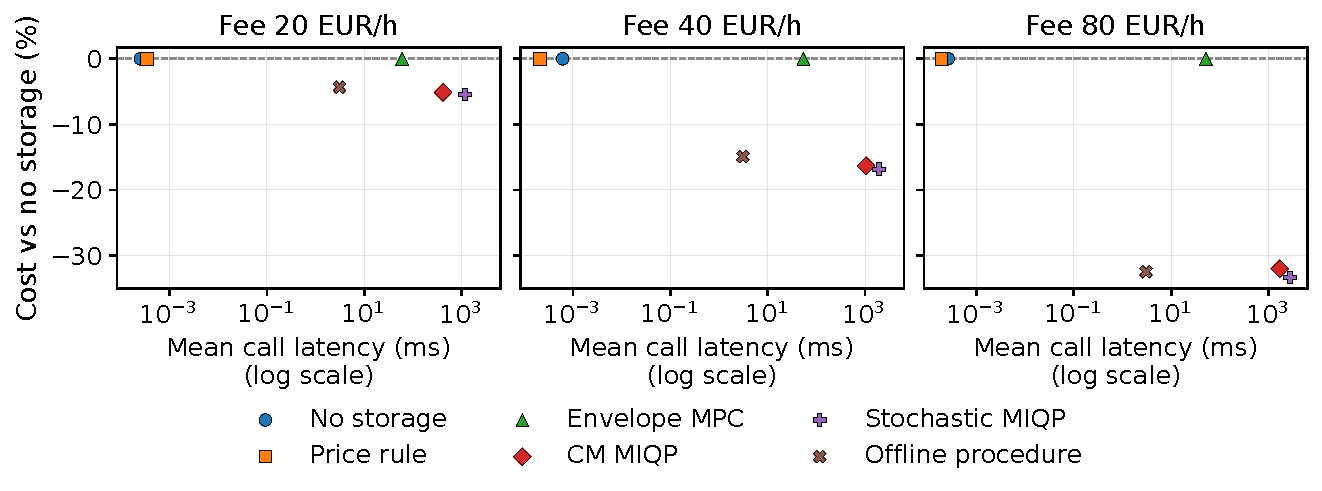
\includegraphics[width=\linewidth]{figures/fig_cost_latency.pdf}
\caption{Operating cost and online computation under the common benchmark. Cost is relative to no storage; latency is measured from controller call to returned held action. Learned evaluation uses the GPU; each MIQP solve uses one CPU thread.}
\label{fig:cost-latency}
\end{figure}

At fee rates of 20, 40, and 80 EUR/h, the offline procedure averaged 1258.2, 1489.1, and 1769.7 EUR/day. These costs were 1.2\%, 2.3\%, and 1.4\% higher, respectively, than the primary two-stage stochastic MIQP (Table~\ref{tab:confirmatory}). The prespecified learned-superiority rule was met in 1 of six MIQP comparisons (Table~\ref{tab:paired}); the supplement reports all baseline comparisons.
The five validation-selected central-fee batch policies ranged from 1485.1 to 1501.1 EUR/day on the common test days.
Zero action was retained in 0 of 7 learned-selection batches. The price-rule baseline selected zero action at all three fees.

A complete five-restart batch required 23.5 minutes of recorded training, validation, and checkpoint loading. Mean online call latency was 3.1 ms, versus 1054.9 ms for conditional-mean MIQP (Figure~\ref{fig:cost-latency}).

\begin{table}[tbp]
\centering
\caption{Primary MIQP comparisons. Differences and bounds are learned minus comparator in EUR/day; fee rates are in EUR/h. The one-sided 95\% upper bound uses paired circular date blocks and, at the central fee, complete training batches. Superiority requires a negative upper bound. Holm $p$ adjusts all 15 comparisons.}
\label{tab:paired}
\small
\begin{tabularx}{\linewidth}{r>{\raggedright\arraybackslash}Xrrrr}
\toprule
Fee & Comparator & Difference & Relative & Upper bound & Holm $p$ \\
\midrule
20 & CM MIQP & 10.3 & 0.8\% & 13.6 & 1.000 \\
20 & Stochastic MIQP & 14.7 & 1.2\% & 17.4 & 1.000 \\
40 & CM MIQP & 24.3 & 1.7\% & 30.3 & 1.000 \\
40 & Stochastic MIQP & 33.1 & 2.3\% & 40.2 & 1.000 \\
80 & CM MIQP & -12.5 & -0.7\% & -6.4 & 0.001 \\
80 & Stochastic MIQP & 23.6 & 1.4\% & 30.1 & 1.000 \\
\bottomrule
\end{tabularx}
\end{table}

\subsection{Value-of-learning attribution}

\begin{table}[tbp]
\centering
\caption{Exploratory attribution to the learned continuation correction. Costs and bounds are in EUR/day and fees in EUR/h. The reference retains the same hard one-step search without the neural correction. Differences are learned minus reference; the one-sided 95\% upper bound resamples five batches at 40 EUR/h and is conditional on one batch at the outer fees.}
\label{tab:reference-attribution}
\resizebox{\linewidth}{!}{%
\begin{tabular}{rrrrrl}
\toprule
Fee & Reference & Learned & Difference & Upper bound & Superiority \\
\midrule
20 & 1295.7 & 1258.2 & -37.5 (-2.9\%) & -31.6 & established \\
40 & 1690.8 & 1489.1 & -201.7 (-11.9\%) & -192.0 & established \\
80 & 2346.2 & 1769.7 & -576.5 (-24.6\%) & -549.7 & established \\
\bottomrule
\end{tabular}
}
\end{table}

The learned continuation reduced cost relative to the reference-only controller at all three anchors, with one-sided upper bounds below zero (Table~\ref{tab:reference-attribution}).
At 40 EUR/h, the learned correction changed the transaction bill by 17.0 EUR/day and degradation by 148.6 EUR/day, while changing the band fee by -367.5 EUR/day. The supplement gives all cost components. Mean controller-call latency across fees was 0.13 ms for the reference controller and 3.08 ms for the learned controller.


\subsection{Mechanisms, seasons, and sensitivity}\label{sec:mechanisms}

The conditional-mean approximation was audited on validation states by
simulating reflected OU transitions. Across weekday regimes and horizons from
1 to 24 hours, the mean absolute difference between the reflected Monte Carlo
mean and the unreflected exponential mean was 0.035--0.164\% of the calibrated
load-error box and 0.041--0.184\% of the price-error box. The largest sampled
absolute differences were 6.06 kW and 0.00097 EUR/kWh. In the held-out 2019
record, 0.057\% of hourly observations lay outside a training box in at least
one error coordinate. These sampled differences are small relative to the
calibrated error ranges.

Across the 27 descriptive factorial cells, the offline policy had lower mean cost than conditional-mean MIQP in 6 cells and lower mean cost than no storage in 27 cells. The three anchors reuse complete five-restart procedures; the other 24 cells use one restart. Width contrasts therefore also reflect unequal selection effort, and the cell counts are descriptive. Realized grid exchange lay within 10 kW of the threshold for 5.77--17.31 hours/day across cells; exact-threshold occupation within $10^{-6}$ kW ranged from 5.76 to 17.31 hours/day. The corresponding mean smooth-minus-hard realized-cost difference ranged from 58.0 to 693.6 EUR/day.

\begin{figure}[t]
\centering
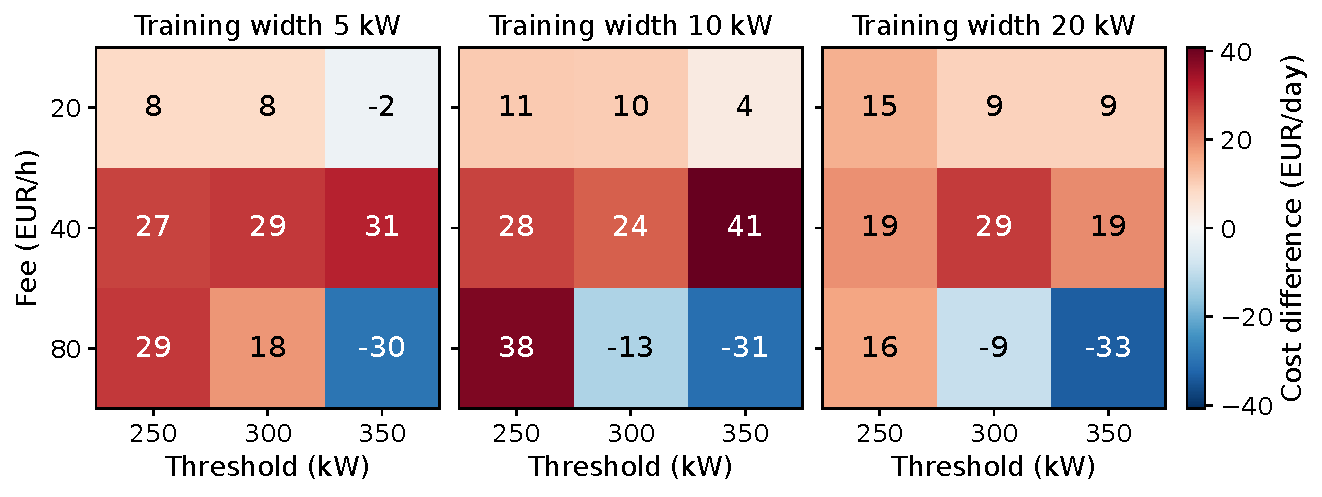
\includegraphics[width=\linewidth]{figures/fig_factorial.pdf}
\caption{Descriptive threshold--fee--smoothing results. Entries are mean offline-minus-conditional-mean-MIQP common costs in EUR/day; negative values favor the offline policy. The three anchors reuse the primary procedures; other cells use one restart.}
\label{fig:factorial}
\end{figure}
% Seasonal and scenario comparisons.
\begin{table}[t]
\centering
\caption{Seasonal replication at 40 EUR/h. Costs are daily means in EUR/day. Winter averages five validation-selected batches; each other season uses one five-restart batch.}
\label{tab:seasons}
\begin{tabular}{lrrrrr}
\toprule
Season & No storage & Convex & CM MIQP & Stoch. MIQP & Offline \\
\midrule
Winter & 1750.6 & 1750.6 & 1464.8 & 1456.0 & 1489.1 \\
Spring & 1342.6 & 1342.7 & 996.1 & 990.9 & 1008.4 \\
Summer & 1232.2 & 1232.3 & 933.4 & 930.9 & 951.7 \\
Autumn & 1345.4 & 1345.5 & 1001.8 & 995.3 & 1049.7 \\
\bottomrule
\end{tabular}
\end{table}

 At the 80 EUR/h anchor, increasing the per-solve limit from 5 to 15 seconds changed mean daily cost by 0.7 EUR for conditional-mean MIQP and -1.4 EUR for two-stage stochastic MIQP; this descriptive sensitivity analysis is separate from the primary comparison. Across the four seasonal regimes, zero action was retained in 0 of 8 complete five-restart batches.

\begin{table}[t]
\centering
\scriptsize
\caption{Exploratory nested scenario-count sensitivity over three fixed streams. Fees are in EUR/h; costs, differences, and bounds are in EUR/day. Costs show the mean [between-stream SD]. Difference is learned minus stochastic MIQP; the one-sided 95\% upper bound resamples paired dates, training batches, and scenario streams. Latency is controller-call mean/mean daily P95; TL is time-limit frequency.}
\label{tab:round2-scenarios}
\begin{tabular}{rrrrrrrr}
\toprule
Fee & $M$ & Limit & MIQP cost [SD] & Difference & Upper & Latency (ms) & TL \\
\midrule
40 & 2 & 5 s & 1456.1 [0.3] & 33.0 & 40.1 & 1953/4468 & 7.8\% \\
40 & 8 & 5 s & 1680.3 [2.5] & -191.1 & -177.8 & 4493/5006 & 78.9\% \\
40 & 16 & 5 s & 1708.1 [0.2] & -218.9 & -203.2 & 4873/5008 & 96.6\% \\
80 & 16 & 5 s & 2469.5 [2.1] & -699.8 & -674.6 & 4857/5009 & 96.8\% \\
80 & 16 & 15 s & 2342.1 [6.2] & -572.4 & -547.7 & 14526/15014 & 96.4\% \\
\bottomrule
\end{tabular}
\end{table}

At 40 EUR/h, increasing the scenario count from 2 to 16 under the fixed five-second budget changed mean stochastic-MIQP cost from 1456.1 to 1708.1 EUR/day; the time-limit frequency changed from 7.8\% to 96.6\%. The learned policy was 218.9 EUR/day less costly than the 16-scenario comparator; its one-sided upper bound was -203.2 EUR/day.
 At 80 EUR/h, the 16-scenario cost changed from 2469.5 to 2342.1 EUR/day when the per-solve limit increased from 5 to 15 seconds. Finite gaps were available for 48.5\% and 97.7\% of calls; their conditional means were 897.50\% and 1167.00\%. These means do not measure matched solver progress because availability and closed-loop states differ. At 15 seconds, the time-limit frequency was 96.4\%. The learned-minus-MIQP upper bound at 15 seconds was -547.7 EUR/day.



\begin{figure}[t]
\centering
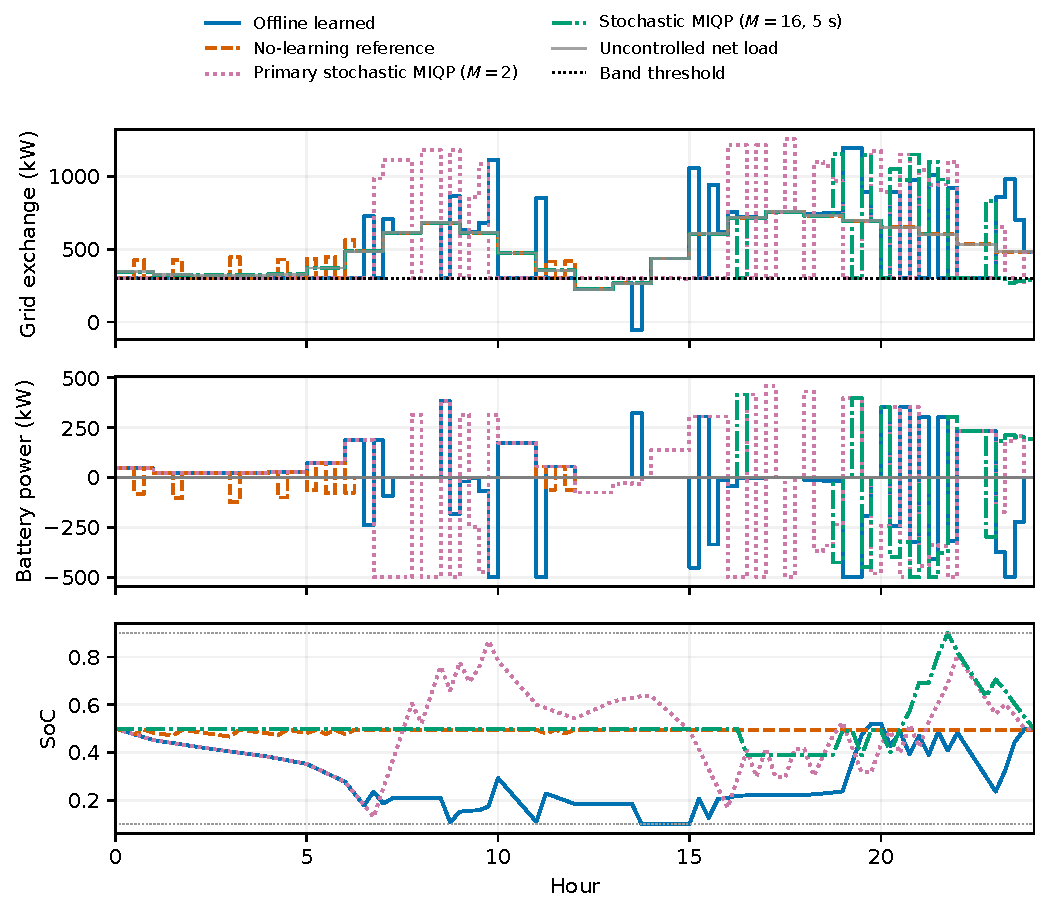
\includegraphics[width=\linewidth]{figures/fig_round2_mechanism.pdf}
\caption{Protocol-selected winter day at 40 EUR/h (7 January 2019):
closest to the median no-storage
exceedance duration, with earliest-date tie breaking. Both stochastic MIQPs
use a 5-s solve limit; the learned curve uses the first validation-selected
batch. Positive battery power denotes discharge.}
\label{fig:round2-mechanism}
\end{figure}
\begin{table}[t]
\centering
\small
\caption{Cost decomposition on the protocol-selected representative winter day (2019-01-07). Costs are in EUR and exceedance duration in hours.}
\label{tab:round2-mechanism}
\resizebox{\linewidth}{!}{%
\begin{tabular}{lrrrrrr}
\toprule
Controller & Bill & Band fee & Degradation & Terminal & Total & Exceed h \\
\midrule
Offline learned policy & 872.3 & 440.0 & 109.1 & 0.08 & 1421.5 & 11.00 \\
No-learning reference controller & 856.1 & 680.0 & 13.5 & 0.27 & 1549.9 & 17.00 \\
Primary stochastic MIQP ($M=2$) & 879.6 & 280.0 & 188.7 & 0.01 & 1348.4 & 7.00 \\
Stochastic MIQP ($M=16$) & 863.8 & 770.0 & 58.4 & 0.01 & 1692.2 & 19.25 \\
\bottomrule
\end{tabular}
}
\end{table}

On this central-fee day (Figure~\ref{fig:round2-mechanism}), the primary
two-scenario MIQP incurred 79.6 EUR more degradation
cost than the learned policy but 160.0 EUR less in band fees, giving 73.1 EUR
lower total cost. The sixteen-scenario procedure instead had the highest cost
among the four displayed policies. The flat fee charges exceedance duration,
not excess power: concentrating imports in fewer above-band intervals can
therefore offset additional cycling cost. The trajectories illustrate this
trade-off within the budgeted procedures.
\FloatBarrier

\section{Computational trade-offs and limitations}\label{sec:compute-economics}

Inference latency alone does not establish an advantage. Let $J_L,J_M$ be
expected daily operating costs for learned and online-optimization policies,
$\tau_L,\tau_M$ their online controller-call seconds per day, $C_{\rm off}$
the monetary value assigned to training and validation, $\kappa_L,\kappa_M$
the respective values of controller-call seconds, and $D$ the number of deployed days between tariff or
site changes. Offline learning breaks even only if
\begin{equation}
 J_L-J_M+\kappa_L\tau_L-\kappa_M\tau_M+\frac{C_{\rm off}}{D}\leq0.
 \label{eq:amortization}
\end{equation}
We report the measurable inputs without assigning a universal compute price.
Retraining after a
tariff change enters $C_{\rm off}$ and shortens $D$.

Against the lower-operating-cost primary stochastic MIQP, learning increases
daily operating cost by 14.7, 33.1, and 23.6 EUR at the three fee anchors.
Under an equal valuation of controller-call seconds, even before charging
for offline work, the saved online computation must
therefore be valued at more than approximately 471, 643, and 321 EUR per
compute-hour, respectively, for a strict economic advantage. These are
break-even valuations, not observed computing prices; actual CPU and GPU
rates can differ. They show why fast
feedback alone does not establish lower total cost; a binding response-time
constraint could instead make latency an operational requirement.

The reference-only counterfactual provides a different comparison. It requires
no neural training and is faster online, but the learned continuation reduces
its daily operating cost by 37.5, 201.7, and 576.5 EUR at the three anchors.
Those savings quantify the economic contribution of learning within the
matched one-step architecture. Whether they justify the additional computation
depends on the deployment duration and its valuation.

Four limitations define the scope. First, the tariff is controlled rather than
a documented customer contract; conclusions concern the optimization
mechanism. Second, OU conditional means are approximate under reflection, and
historical errors need not be Gaussian or Markov. Third, two-stage stochastic
MIQP grants scenario-contingent future recourse and is not a multistage policy.
Fourth, neural results remain training-batch dependent even after economic
selection. The exact-band label describes
the mixed-integer formulation, not the status of every online solve. Increasing
the scenario count changes both the stochastic approximation and the difficulty
of the budgeted optimization. Scenario and budget comparisons therefore
concern implemented procedures, not globally solved stochastic control.

\section{Conclusion}\label{sec:conclusion}

The simulation study compares offline value learning and online mixed-integer
MPC as complete decision procedures under matched deployment rules. On 30 held-out winter
weekdays, the offline procedure cost 1.2\%, 2.3\%, and 1.4\% more than the
lower-cost primary stochastic MIQP at fee rates of 20, 40, and 80 EUR/h.
Its mean online latency was 3.1 ms, with 23.5 minutes of measured offline
work per five-restart batch. Only the high-fee comparison with conditional-mean
MIQP met the prespecified learned-superiority rule. Central-fee inference
includes five independent five-restart batches; the outer-fee comparisons
are conditional on one batch each. At the central fee, the stochastic MIQP
also had lower mean cost in every season, with learned-policy premiums
ranging from 1.8\% in spring to 5.5\% in autumn.

The matched reference-value controller separates the hard one-step search
from the learned continuation correction. Relative to this no-learning rule,
the correction reduced cost by 2.9\%, 11.9\%, and 24.6\% at the three fee
anchors, with one-sided upper bounds below zero. Learning thus contributes
within the matched one-step architecture, while the primary stochastic
MIQP achieves lower operating cost. These are distinct findings.

The reference-policy ansatz and hard one-step deployment address two avoidable
sources of learned-policy error. The discrete Bellman result then separates
residual variation, held-action defect, numerical expectation error, and
terminal approximation. For the threshold-tariff dispatch problem studied
here, choosing between offline learning and online optimization requires
jointly assessing operating cost, online computation, and the deployment
period over which training costs are amortized.

\section*{CRediT authorship contribution statement}

Yeoneung Kim: Conceptualization, Methodology, Software, Validation, Formal
analysis, Investigation, Data curation, Writing--original draft,
Writing--review and editing, and Visualization.

\section*{Supplementary material}

The supplementary material provides the evaluation protocol, calibration
parameters, mixed-integer formulations, learning and deployment details,
numerical checks, and additional results.

\section*{Data availability}

The source data are available from Open Power System Data \citep{OPSD2020}. Code, processed
inputs, stored model weights, and the reported evaluation outputs are
available in the GitHub repository at \url{https://github.com/yeoneung/rvpinn}.
The code, numerical results, and accompanying manuscript are provided in
\href{https://github.com/yeoneung/rvpinn/tree/v1.0.0}{version \texttt{1.0.0}} \citep{KimDispatch2026}.

\section*{Declaration of competing interest}

The author declares no competing interests.

\section*{Declaration of generative AI and AI-assisted technologies in the
manuscript preparation process}

During the preparation of this work, the author used OpenAI Codex to assist
with language editing, manuscript organization, code review, and the
preparation of experiment and visualization scripts. After using this tool,
the author reviewed and edited the content as needed and takes full
responsibility for the content of the publication.

\section*{Acknowledgements}

Funding: This work was supported by the National Research Foundation of Korea (NRF)
grants funded by the Korea government (MSIT)
[grant numbers RS-2023-00219980, RS-2026-25490291]; and Yonsei University.
The funders had no role in the study design; data collection, analysis, or
interpretation; manuscript preparation; or the decision to submit the
article for publication.

\bibliographystyle{elsarticle-num-names}
\bibliography{references}

\end{document}
